\documentclass{article} % For LaTeX2e
\usepackage{nips14submit_e,times}
\usepackage{amsmath}
\usepackage{amsthm}
\usepackage{amssymb}
\usepackage{mathtools}
\usepackage{hyperref}
\usepackage{url}
\usepackage{algorithm}
\usepackage[noend]{algpseudocode}
%\documentstyle[nips14submit_09,times,art10]{article} % For LaTeX 2.09

\usepackage{bbm}
\usepackage{graphicx}
\usepackage{caption}
\usepackage{subcaption}
\usepackage{MnSymbol}

\def\eQb#1\eQe{\begin{eqnarray*}#1\end{eqnarray*}}
\def\eQnb#1\eQne{\begin{eqnarray}#1\end{eqnarray}}
\providecommand{\e}[1]{\ensuremath{\times 10^{#1}}}
\providecommand{\pb}[0]{\pagebreak}
\DeclarePairedDelimiter\ceil{\lceil}{\rceil}
\DeclarePairedDelimiter\floor{\lfloor}{\rfloor}

\newcommand{\E}{\mathrm{E}}
\newcommand{\Var}{\mathrm{Var}}
\newcommand{\Cov}{\mathrm{Cov}}
\newcommand\eqD{\stackrel{\mathclap{\normalfont\mbox{d}}}{=}}

\def\Qb#1\Qe{\begin{question}#1\end{question}}
\def\Sb#1\Se{\begin{solution}#1\end{solution}}

\newenvironment{claim}[1]{\par\noindent\underline{Claim:}\space#1}{}
\newtheoremstyle{quest}{\topsep}{\topsep}{}{}{\bfseries}{}{ }{\thmname{#1}\thmnote{ #3}.}
\theoremstyle{quest}
\newtheorem*{definition}{Definition}
\newtheorem*{theorem}{Theorem}
\newtheorem*{lemma}{Lemma}
\newtheorem*{question}{Question}
\newtheorem*{preposition}{Preposition}
\newtheorem*{exercise}{Exercise}
\newtheorem*{challengeproblem}{Challenge Problem}
\newtheorem*{solution}{Solution}
\newtheorem*{remark}{Remark}
\usepackage{verbatimbox}
\usepackage{listings}
\usepackage{mathrsfs}
\title{ProbLimI: \\
Problem Set X}


\author{
Youngduck Choi \\
CIMS \\
New York University\\
\texttt{yc1104@nyu.edu} \\
}


% The \author macro works with any number of authors. There are two commands
% used to separate the names and addresses of multiple authors: \And and \AND.
%
% Using \And between authors leaves it to \LaTeX{} to determine where to break
% the lines. Using \AND forces a linebreak at that point. So, if \LaTeX{}
% puts 3 of 4 authors names on the first line, and the last on the second
% line, try using \AND instead of \And before the third author name.

\newcommand{\fix}{\marginpar{FIX}}
\newcommand{\new}{\marginpar{NEW}}

\nipsfinalcopy % Uncomment for camera-ready version

\begin{document}


\maketitle

\begin{abstract}
This work contains solutions to the exercises of the problem set X. The
chosen problems are 1,3,4.
\end{abstract}

\bigskip


\begin{question}[1]
\hfill
\begin{figure}[h!]
  \centering
    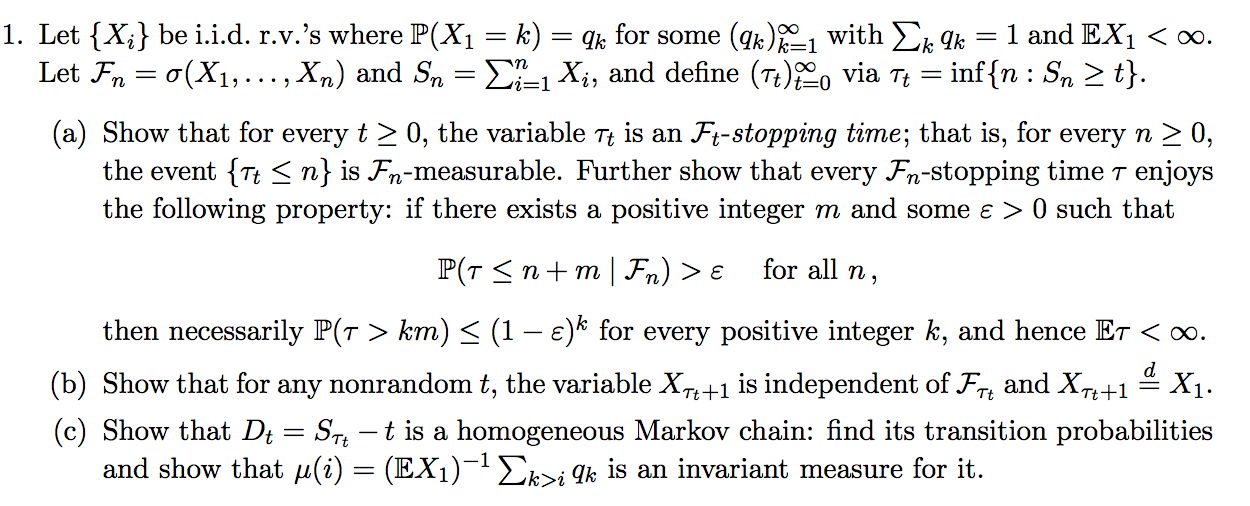
\includegraphics[width=0.7\textwidth]{prob-e10-p1.png}
\end{figure}
\end{question}
\begin{solution} \hfill \\
\textbf{(a)} Observe that
\eQb
\{\tau_{t} \leq n \} &=& \{ \inf\{m \geq 1 \> : \> S_m \geq t \} \leq n \} \\
&=& \bigcup_{m=1}^{n} \{S_m \geq t \} \in \sigma(X_1,...,X_n) = \mathscr{F}_n 
\eQe
for any $n \geq 1$ and $t \geq 0$, and hence $\tau_t$ is an $\mathscr{F}_t$ 
measurable. 

\smallskip

Suppose $\tau$ is a $\mathscr{F}_n$ stopping time and there exists a positive integer
$m$ and $\epsilon > 0$ such that
\eQb
\mathbb{P}(\tau \leq n + m \> | \> \mathscr{F}_n) > \epsilon
\eQe
for all $n \geq 1$. 


\end{solution}

\newpage

\begin{question}[2]
\hfill
\begin{figure}[h!]
  \centering
    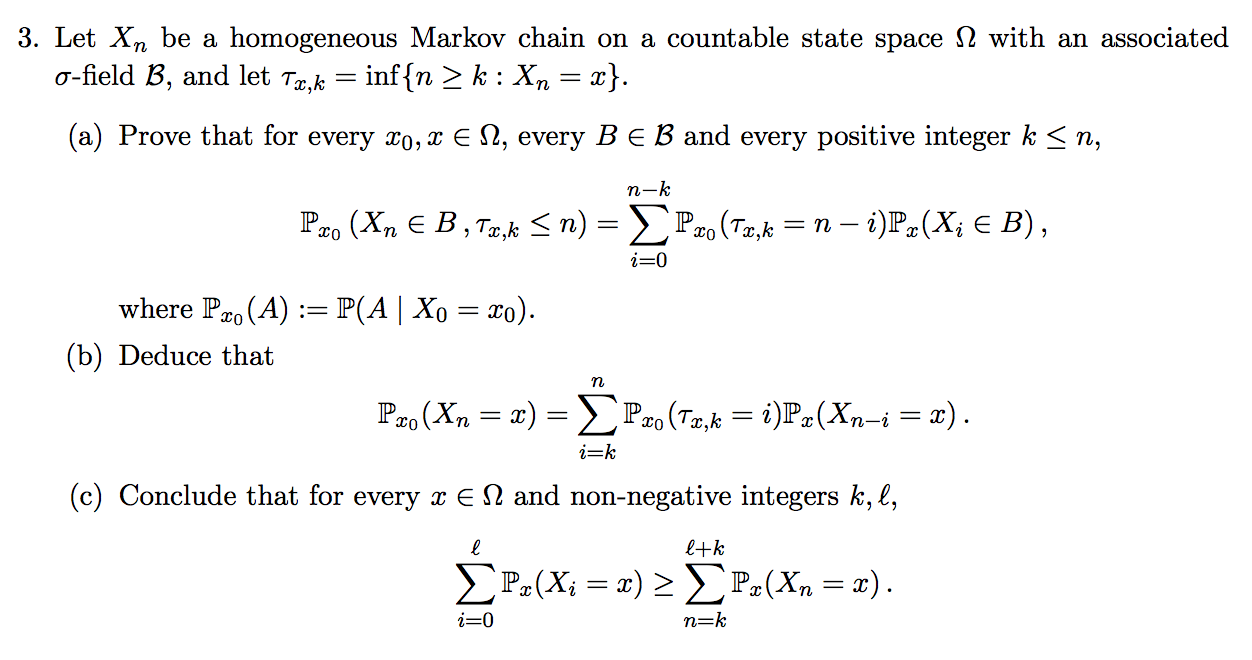
\includegraphics[width=0.7\textwidth]{prob-e10-p2.png}
\end{figure}
\end{question}
\begin{solution} \hfill \\
\textbf{(a)} 
By homogeneity,
\eQb
\mathbb{P}_x(X_i \in B) = 
\mathbb{P}(X_i \in B | X_0 = x) = \mathbb{P}(X_n \in B | X_{n-i} = x) 
\eQe
for any $1 \leq i \leq n$. Then, 
\eQb
\mathbb{P}_{x_0}(X_n \in B , \tau_{x,k} \leq n) &=& 
\mathbb{P}_{x_0}(\bigcup_{i=0}^{n-k} X_n \in B , \tau_{x,k} = n-i) \\
&=& \sum_{i=0}^{n-k} \mathbb{P}_{x_0}( X_n \in B , \tau_{x,k} = n-i) \\
&=&
\sum_{i=0}^{n-k} \mathbb{P}_{x_0}(\tau_{x,k} = n-i)\mathbb{P}(X_n \in B | X_{n-i} = x)
\\ 
&=& 
\sum_{i=0}^{n-k} \mathbb{P}_{x_0}(\tau_{x,k} = n-i)\mathbb{P}_{x}(X_i \in B). 
\eQe

\bigskip

\textbf{(b)} In view of (a), setting $B = \{x\}$,
\eQnb
\mathbb{P}_{x_0}(X_n = x)
&=& \mathbb{P}_{x_0}(X_n = x, \tau_{x,k} \leq n) \label{eq:1} \\
&=& \sum_{i=k}^{n} 
\mathbb{P}_{x_0}(\tau_{x,k} = i)\mathbb{P}_x(X_{n-i} = x) \nonumber 
\eQne
where~\eqref{eq:1} holds as $\{X_n = x\} \subset \{ \tau_{x,k} \leq n \}$. 

\bigskip

\textbf{(c)} Applying (b) with $x_0 = x$,  
\eQnb
\sum_{n=k}^{l+k} \mathbb{P}_x(X_n = x) &=& 
\sum_{n=k}^{l+k} \sum_{i=k}^{n} \mathbb{P}_x(\tau_{x,k} = i) 
\mathbb{P}_x(X_{n-i} = x) \nonumber \\ 
&=& \sum_{i=0}^{l} \mathbb{P}_x( X_i = x) \sum_{i=k}^{n-j} \mathbb{P}_x(
\tau_{x,k} = i) \nonumber \\
&\leq& \sum_{i=0}^{l} \mathbb{P}_x( X_i = x) \label{eq:3} 
\eQne
where~\eqref{eq:3} holds by disjointness. \hfill $\qed$ 

\end{solution}

\newpage

\begin{question}[3]
\hfill
\begin{figure}[h!]
  \centering
    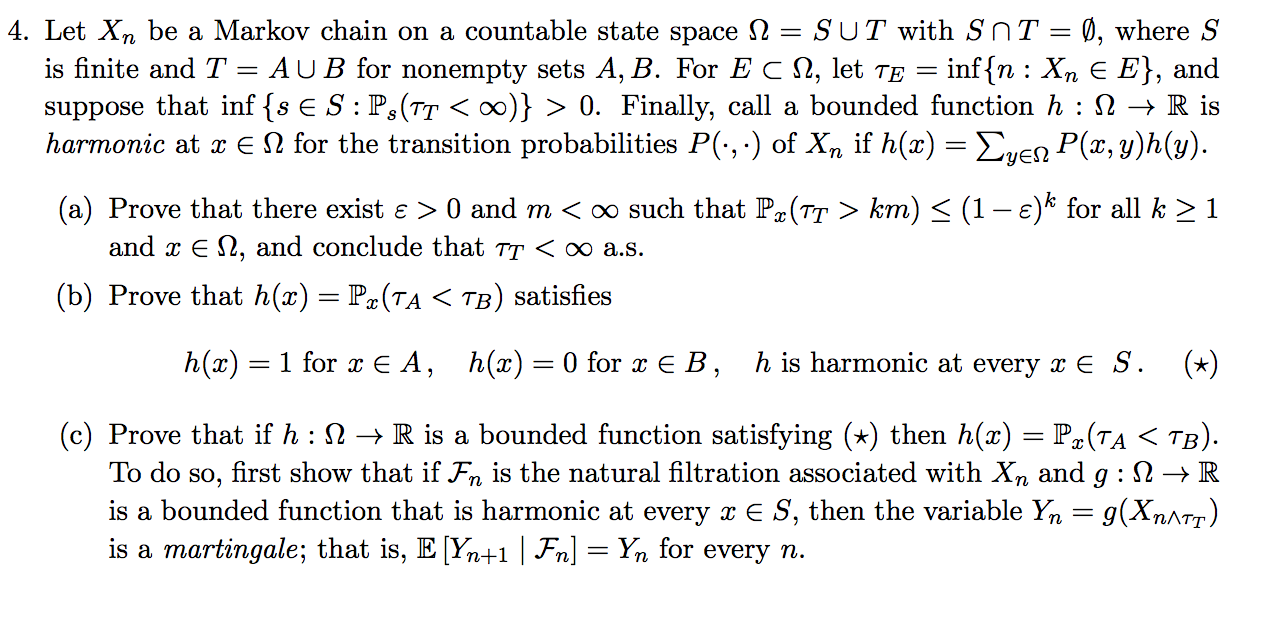
\includegraphics[width=0.7\textwidth]{prob-e10-p3.png}
\end{figure}
\end{question}
\begin{solution} \hfill \\
\textbf{(a)}
We claim that
\eQb
\mathbb{P}(X_i \in B | X_0 = x) = \mathbb{P}(X_n \in B | X_{n-i} = x) 
\eQe
for any $n \geq 1$ and $n \geq i \geq 1$. We proceed by induction on $i$. Then,
\eQb
\mathbb{P}_{x_0}(X_n \in B , \tau_{x,k} \leq n) &=& 
\mathbb{P}_{x_0}(\bigcup_{i=0}^{n-k} X_n \in B , \tau_{x,k} = n-i) 
\eQe 

\bigskip

\textbf{(b)}


\bigskip



\end{solution}
\end{document}


